\section{Feedback Task Offloading}
\label{sec:PADLB-FeedbackLB}
\index{PADLB!Feedback Task Offloading}

The idea behind feedback is an improvement of reactive approach. Applying to iterative applications, the first iteration is kept doing with reactive load balancing. Tasks are offloaded from a slow process to a fast one during execution. After the first iteration, we use $Tcomm$ to generate a statistic on each process about the number of executed tasks in local and remote processes, the total load values of local and remote tasks. The statistic shows how good balancing in the first iteration is. Then, we use this statistic to interpolate the load difference among processes that support an estimation for which processes are overloaded and underloaded. From here, a priority function for task offloading is generated as feedback to drive proactive task offloading in the next iterations.\\

\begin{figure}[t]
	\centering
	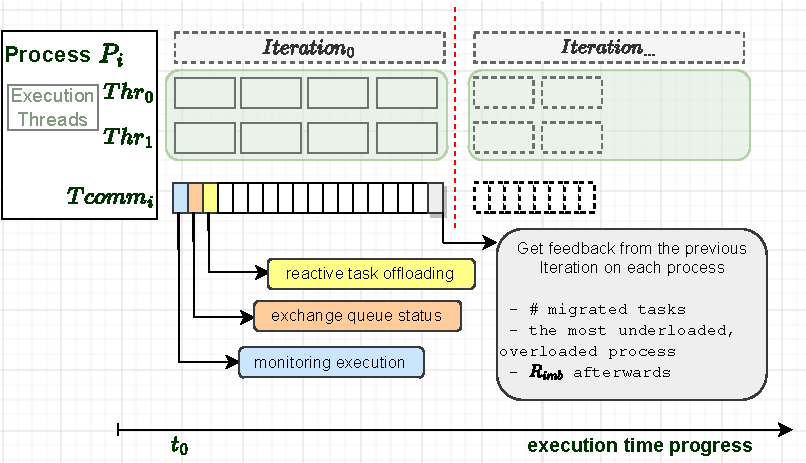
\includegraphics[scale=0.65]{./pictures/padlb_approach/padlb_feedback_lb_idea.pdf}
	\caption{An overview of feedback task offloading through the operations of $Tcomm$.}
	\label{fig:padlb_feedback_task_offloading}
\end{figure}

Figure \ref{fig:padlb_feedback_task_offloading} presents the design of $Tcomm$ to perform feedback task offloading. Again with the coordinates, the x-axis indicates execution time progress. Vertically, we illustrate process $P_{i}$, where its two main threads ($Thr_{0}$, $Thr_{1}$) are shown with executing tasks, $Tcomm_{i}$ with balancing operations. In the first iteration ($Iteration_{0}$), the operations of reactive load balancing are performed the same. For instance, we can see the small rectangles with three different colors. Each rectangle represents an operation in reactive load balancing, where blue is monitoring execution (i.e., queue length), orange is exchanging the status, and yellow is offloading tasks. These operations are repeated until $Iteration_{0}$ is terminated. From here, the arrow at the last rectangle on $Tcomm_{i}$ points to a statistic for feedback.\\

A crucial question is what information is needed for feedback. In this method, we collect the information regarding the efficiency of the first iteration, including:

\begin{itemize}
	\item The number of local and remote tasks executed in a process.
	\item The number of offloaded tasks.
	\item The total load values of local and remote tasks.
	\item The $R_{imb}$ ratio and speed up after reactive load balancing in the first iteration.
\end{itemize}

\begin{algorithm}[t]
\caption{Feedback Task Offloading} \label{alg:feedback_task_offloading}
	\setstretch{1.25}		% for the spacing between lines
	\DontPrintSemicolon % for not showing the semicolon of an empty line command
	\SetNoFillComment		% to align the comment position
	\SetKwInOut{KwIN}{Input}
	\SetKwInOut{KwOUT}{Output}
	\SetKwInOut{KwRET}{Return}
	
	\SetKwFunction{FBba}{feedback\_balancing}
	\SetKwFunction{ASer}{assert}
	\SetKwFunction{EVal}{evaluate}

	% --------------------------------------------
	\; % intended for an empty line as spacing
  % --------------------------------------------
  \KwIN{Array $L^{\text{local}}$\texttt{[]}, $L^{\text{remote}}$\texttt{[]}, $N^{\text{local}}$\texttt{[]}, $N^{\text{remote}}$\texttt{[]}, each has P elements. Where, $L^{\text{local}}\texttt{[i]}$ is local load value; \\
  		$L^{\text{remote}}\texttt{[i]}$ is remote load value; \\
  		$N^{\text{local}}\texttt{[i]}$ is the number of local tasks; and \\
  		$N^{\text{remote}}\texttt{[i]}$ is the number of remote tasks in process $P_{i}$}
  \KwOUT{Array $D_{\text{reference}}\texttt{[]}$: a reference distribution of priorities}
  % --------------------------------------------
	\; % intended for an empty line as spacing
  % --------------------------------------------
  \SetKwProg{Fn}{Procedure}{:}{}
  \Fn{\FBba{\texttt{Array} $L^{\text{local}}$, $L^{\text{remote}}$, $N^{\text{local}}$, $N^{\text{remote}}$}}{
  	\tcc{Check the input}
  	\nl \ASer{$L^{\text{local}}$, $L^{\text{remote}}$, $N^{\text{local}}$, $N^{\text{remote}}$} \\
  	\nl \ASer{$\texttt{flag}_{\text{feedback}}$} \\
		% --------------------------------------------
		\; % intended for an empty line as spacing
		% --------------------------------------------
  	\tcc{Summarize statistic}
		\nl \texttt{Array} $L$ $\leftarrow$ $L^{\text{local}}$ $+$ $L^{\text{remote}}$  \\
		\nl $L_{max}$, $L_{avg}$ $\leftarrow$ maximum and average load based on Array $L$ \\
		\nl $R_{imb}$ $\leftarrow$ calculate imbalance ratio in overall \\
		\nl \EVal{$R_{imb}$} \tcp*[l]{evaluate the efficiency of reactive load balancing in the first/previous iteration}
		% --------------------------------------------
		\; % intended for an empty line as spacing
		% --------------------------------------------
		\tcc{Interpolate the original load values and local tasks based on average}
		\nl \For{$i \leftarrow 0$ \KwTo \texttt{P-1}}{
				\nl $\hat{L}\texttt{[i]}$, $\hat{w}^{\text{local}}\texttt{[i]}$ $\leftarrow$ based on $L^{\text{local}}\texttt{[i]}$, $N^{\text{local}}\texttt{[i]}$ \\
				\nl $\hat{w}^{\text{remote}}\texttt{[i]}$ $\leftarrow$ based on $L^{\text{remote}}\texttt{[i]}$, $N^{\text{remote}}\texttt{[i]}$ \\
		}
		\nl $\hat{L}_{max}$, $\hat{L}_{avg}$ $\leftarrow$ maximum and average load based on \texttt{Array} $\hat{L}$ \\
		\nl $\hat{R}_{imb}$ $\leftarrow$ calculated by $\hat{L}_{max}$, $\hat{L}_{avg}$ \\
		\nl $D_{\text{reference}}$ $\leftarrow$ a reference distribution of priorities if $\hat{R}_{imb}$ $\geq$ $\texttt{Threshold}_{\texttt{imb}}$ \\
		
%		\nl \If{$\hat{R}_{imb} \geq \texttt{Threshold}_{\texttt{imb}}$}{
%				\nl $D_{\text{reference}}[]$ $\leftarrow$ a reference distribution of priorities \\
%		}

		\nl \KwRET{$D_{\text{reference}}$}
  }
  
  % --------------------------------------------
	%\; % intended for an empty line as spacing
  % --------------------------------------------
	%\SetKwProg{Fn}{Procedure}{:}{}
  %\Fn{\FCoo{\texttt{Array} $\texttt{IDLE}^{'}$}}{
  	%\tcc{Check runtime information}
		%\nl $pid$ $\leftarrow$ check process id \\
		%\nl $B$ $\leftarrow$ check average bandwidth information for task migration \\
			
		% --------------------------------------------
		%\; % intended for an empty line as spacing
		% --------------------------------------------
		%\KwRET{$P_{\texttt{victim}}$, $\texttt{num}_{\texttt{offload}}$}
  %}
\end{algorithm}

In case the current iteration is not the first iteration (\texttt{Iteration 0}), feedback requests the iteration called the \textit{previous} iteration. Generally, Algorithm \ref{alg:feedback_task_offloading} shows how the feedback information works on each process. The feedback includes recorded information about the local, remote load, number of local tasks, and number of remote tasks denoted by $L^{\text{local}}$\texttt{[]}, $L^{\text{remote}}$\texttt{[]}, $N^{\text{local}}$\texttt{[]}, $N^{\text{remote}}$ \texttt{[]} respectively. The output is an array of priorities corresponding to each process. The priority gives each a reference number that says offloading tasks (if $> 0$) or receiving tasks (if $< 0$). Their values suggest a reference limit for how many tasks we should offload or receive in a process. These input/output arrays have $P$ elements alluding to the number of involved processes.\\

(1) Procedure \texttt{feedback\_balancing()} checks the input arrays. Then, it is ensured to run only one time every iteration by the flag $\texttt{flag}_{\text{feedback}}$, except for the first iteration of collecting data to give feedback.\\

(2) We summarize a statistic about how good reactive load balancing is performed in the first/previous iteration.\\

The total load value ($L$) per process is calculated by the sum of local and remote load, $L^{\text{local}}$ $+$ $L^{\text{remote}}$. After distributing the values $L$, $L^{\text{local}}$, $L^{\text{remote}}$ around, each process calculates $L_{max}$, $L_{avg}$ that are used to check the imbalance ratio $R_{imb}$. By evaluating $R_{imb}$, we can determine the efficiency of reactive load balancing in the first/previous iteration.\\

(3) The procedure interpolates information about the original load value and task execution time of each process based on average, denoted by $\hat{L}\texttt{[i]}$, $\hat{w}^{\text{local}}\texttt{[i]}$. Also, if the current process executed remote tasks, the corresponding $\hat{w}^{\text{remote}}\texttt{[i]}$ is also estimated. Benefit from $\hat{L}$, we estimate information about $\hat{L}_{max}$, $\hat{L}_{avg}$ $\hat{R}_{imb}$ to check how load difference among processes if reactive load balancing is not applied. Eventually, the difference of $\hat{L}$ and $\hat{L}_{avg}$ associated with $\hat{w}^{\text{local}}\texttt{[i]}$ and $\hat{w}^{\text{remote}}\texttt{[i]}$ supports generating an array of priorities, $D_{\text{reference}}$. As a result, we interpolate the number of tasks that should be offloaded/received to fill the gap between $\hat{L}$ and $\hat{L}_{avg}$. For example, process $P_{i}$ has $D_{\text{reference}}\texttt{[i]} = 99$ that says it should be an offloader, and a reference limit is $99$ tasks.\\

An obvious advantage in feedback task offloading is determining which process is a potential victim for offloading tasks and which is receiving tasks. Another advantage is that we can refer to a limit of how many tasks should be offloaded. These points can drive task offloading in subsequent iterations better.

%In detail, we still rely on the operations of reactive load balancing. However, after each execution phase, we review the progress and use statistics to give feedback for offloading tasks in the next iterations. This can leverage the offloading operations to be more proactive about which processes can potentially be victims. \\

%As we can see in Figure \ref{fig:padlb_feedback_load_balancing}, the first iteration remains reactive task offloading operations. $Tcomm_{i}$ repeatedly monitors each process's queue status, exchanges that information around, and offloads tasks reactively if the imbalance ratio meets. After that, all task offloading data will be recorded for analysis. We make statistics about:


